\chapter{Experimental Setup} \label{chap:exp_setup}

\section{Vortex Configuration}

Section~\ref{sec:gpu_simulation} explained how \acrshort{fpga}-accelerated simulations have to correctly scale memory bandwidth and latency to obtain representative results. As work is still being done at NTNU to integrate \Gls{vortex} into chipyard~\cite{chipyard}, I have to use software simulations. The Vortex project has a built-in script for running benchmarks. The script allows for setting several parameters and configurations for the benchmarks, architecture and simulator. \Gls{vortex}' simulation stack, includes four simulation environments shown in Figure~\ref{fig:simstack}. In this thesis, I use \textit{VLSIM}. VLSIM use Verilator~\cite{verilator} to simulate the full RTL design and implements the accelerator functional unit (AFU) interface in software. Memory is also simulated in software using Ramulator~\cite{Ramulator}. The configurations I used are listed in Table~\ref{tab:vortex_config}, while the benchmarks are listed in Table~\ref{tab:benchmarks}. The number of warps and threads per \acrshort{sm} is based on \Gls{vortex}' default configuration. In my project thesis~\cite{Aurud_Project}, I tested a range of configurations with different numbers of \acrshortpl{sm} and found that all benchmarks worked as intended for up to 32 \acrshortpl{sm}. For 64 \acrshortpl{sm}, some of the benchmarks returned erroneous results. Because of this, I elected to continue evaluating Vortex with 32 \acrshortpl{sm}.

% -- Simulation stack
\begin{figure}
    \centering
    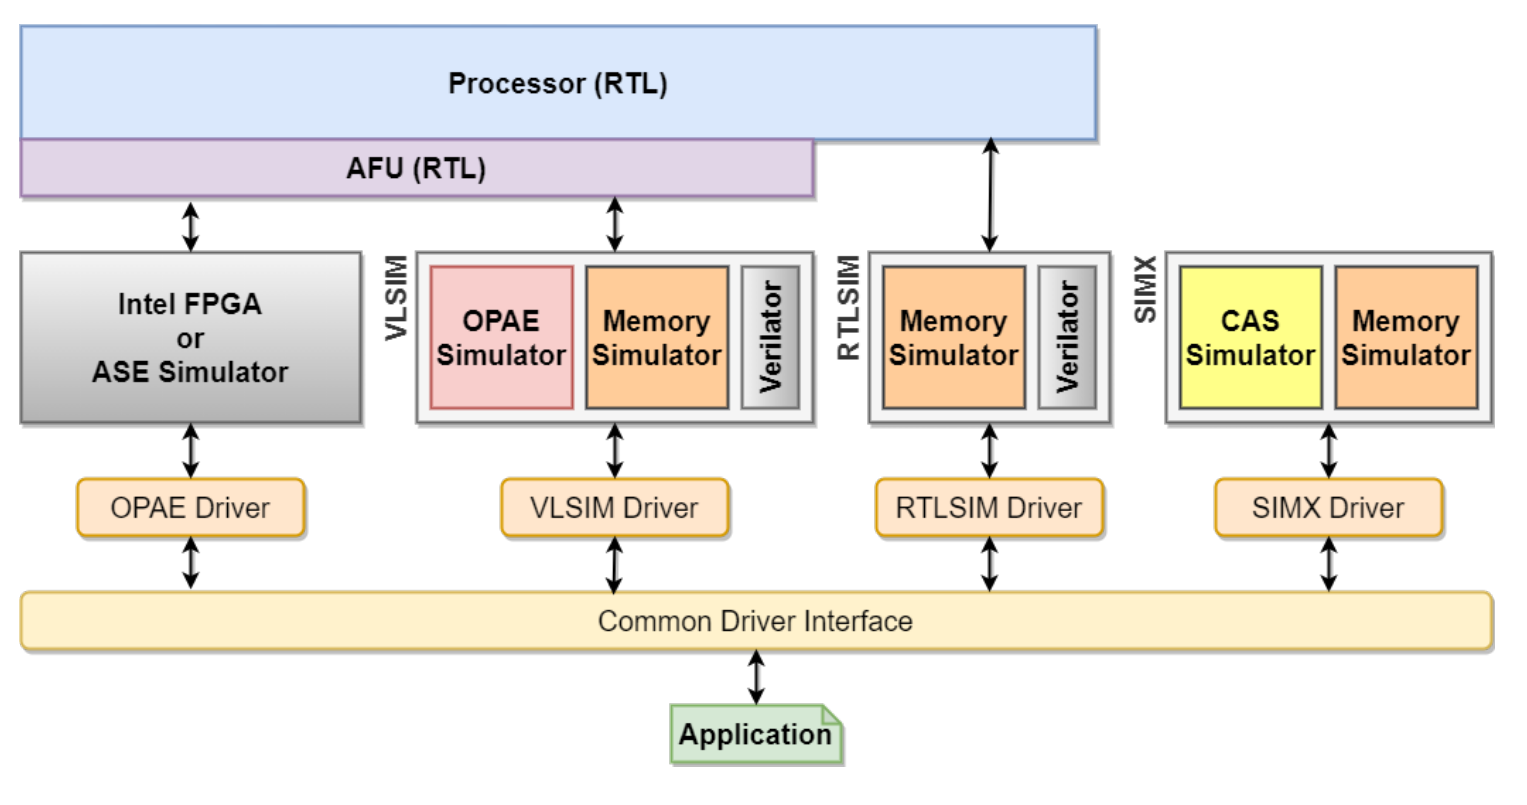
\includegraphics[width=0.8\textwidth]{figures/simstack.png}
    \caption[Vortex simulation stack]{Vortex simulation stack reproduced from~\cite{vortex}.}
    \label{fig:simstack}
\end{figure}

% -- Table of Vortex Configurations
\begin{table}
    \centering
    \caption{Configurations for the Vortex architecture.}
    \begin{tabular}{|l|l|} 
    \hline
    \multicolumn{2}{|c|}{\textbf{Vortex Configuration}} \\ \hline
     
    \makecell[l]{GPU} & \makecell[l]{32 cores, 1.2GHz, 16 threads/\acrshort{sm}, \\ 4 threads/warp, 4 warps/\acrshort{sm}} \\ \hline

    \makecell[l]{Clustering} & \makecell[l]{8 cores/cluster (4 clusters)} \\ \hline
     
    \makecell[l]{GPU L1 Cache} & \makecell[l]{16KiB per \acrshort{sm}, direct mapped, \\ 16B blocks, 4B words} \\ \hline

    \makecell[l]{GPU L2 Cache} & \makecell[l]{128KiB per cluster, direct mapped \\ 64B blocks} \\ \hline

    \makecell[l]{GPU L3 Cache} & \makecell[l]{No L3 cache} \\ \hline

    \makecell[l]{DDR4} & \makecell[l]{DDR4 2400R (1200 MHz), 19.2GB/s, \\ 4Gbx8, 1 channel, 1 rank/channel \\ $t_{CL}=16$, $t_{RCD}=16$, $t_{RP}=16$} \\ \hline
     
    NoC & Hierarchical tree structure \\ \hline
    \end{tabular}
    \label{tab:vortex_config}
\end{table}

% -- Table of benchmarks
\begin{table}
    \centering
    \caption[Overview of benchmarks and the adjusted input sizes.]{Overview of benchmarks and the adjusted input sizes. The first 6 benchmarks are the benchmarks not ported by me}
    \begin{tabular}{|l|l|l|l|} 
        \hline
        \makecell[l]{\textbf{Benchmark}}         & \makecell[l]{\textbf{Short} \\ \textbf{Name}} & \makecell[l]{\textbf{Default} \\ \textbf{Input Size}}    & \makecell[l]{\textbf{Adjusted} \\ \textbf{Input Sizes}} \\ \hhline{|=|=|=|=|}
        Vector Addition            & Vecadd        & 64                             & 32768              \\ \hline
        General Matrix Multiply    & Sgemm         & 32x32 Matrix                   & 256x256 Matrix          \\ \hline
        Matrix Filter (3x3 kernel) & Sfilter       & 16                             & 1024         \\ \hline
        Sorting                    & Psort         & 16                             & 8192  \\ \hline
        A times X plus Y           & Saxpy         & 16                             & 262144 ($2^{18}$)  \\ \hline
        Nearest Neighbour Search   & Nearn         & 40k Records                    & - \\ \hhline{|=|=|=|=|}
        B+ Tree Graph Traversal    & B+tree        & 1M Elements                    & 10K Elements \\ \hline
        Back propogation           & Backprop      & 65536                          & - \\ \hline
        Breadth-First Search       & BFS & 4096 Nodes                               & 65536 Nodes  \\ \hline
        CFD Solver                 & CFD & fvcorr.domn.097K                         & missile.domn.0.2M  \\ \hline
        GPUDWT                     & DWT2D & 192x192 Bitmap                         & -  \\ \hline
        Gaussian elimination       & Gaussian      & 16x16 Matrix                   & 512x512 Matrix \\ \hline
        Heart Wall                 & HW            & 20 Frames                      & - \\ \hline
        HotSpot                    & Hotspot       & 512 2 2                        & 512 2 2  \\ \hline
        HotSpot3D                  & 3D            & 512 8 100                      & 512 8 4  \\ \hline
        \makecell[l]{Kmeans}                     & \makecell[l]{Kmeans} & \makecell[l]{100 Points,\\100 Features}       & \makecell[l]{2048 Points \\ 128 Features} \\ \hline
        LavaMD2                    & LavaMD        & -boxes1d 10                    & -boxes1d 16 \\ \hline
        LU Decomposition           & LUD           & 1024x1024 Matrix                         & -  \\ \hline
        \makecell[l]{Needleman-Wunsch}           & \makecell[l]{NW}            & \makecell[l]{2048x2048 Matrix \\ 10 Penalty}     & \makecell[l]{-}  \\ \hline
        SRAD                       & SRAD          & 502x458 Image                  & 251x229 Image  \\ \hline
        Streamcluster              & SC            & 65536 Points                   & - \\ \hline
    \end{tabular}
    \label{tab:benchmarks}
\end{table}

\section{Benchmarks}
In my project thesis \cite{Aurud_Project}, I found that the benchmarks included by \Gls{vortex} required a much larger input size than the default to give reasonable performance results. That is, having enough work to have realistic memory usage and to activate all the \acrshortpl{sm}. The adjusted input sizes, as well as the inputs for the new benchmarks, are displayed in Table \ref{tab:benchmarks}.
\newpage
To keep the simulation time reasonable, I implemented fast-forward, warm-up and early-exit, as described in Section~\ref{sec:ff_wu_ee}. To do this, I have to find how many cycles are required for the caches to become warm and get past the startup. Figure~\ref{fig:l1_cache_startup_hitrate} and \ref{fig:l2_cache_startup_hitrate} respectively show the cache hit rate during startup of the L1 and L2 caches when running a subset of the benchmarks. After 30k cycles, the cache hit rates are stabilizing for both the L1 and L2 caches. While the L1 hit rate for \textit{backprop} is fluctuating, it is probably due to its access pattern. To have some extra margins, I chose to use 50k fast-forward and warm-up cycles. For early-exit, I let the benchmarks run for up to 10M cycles before terminating.

\begin{figure}
    \centering
    \begin{subfigure}[t]{\textwidth}
        \centering
        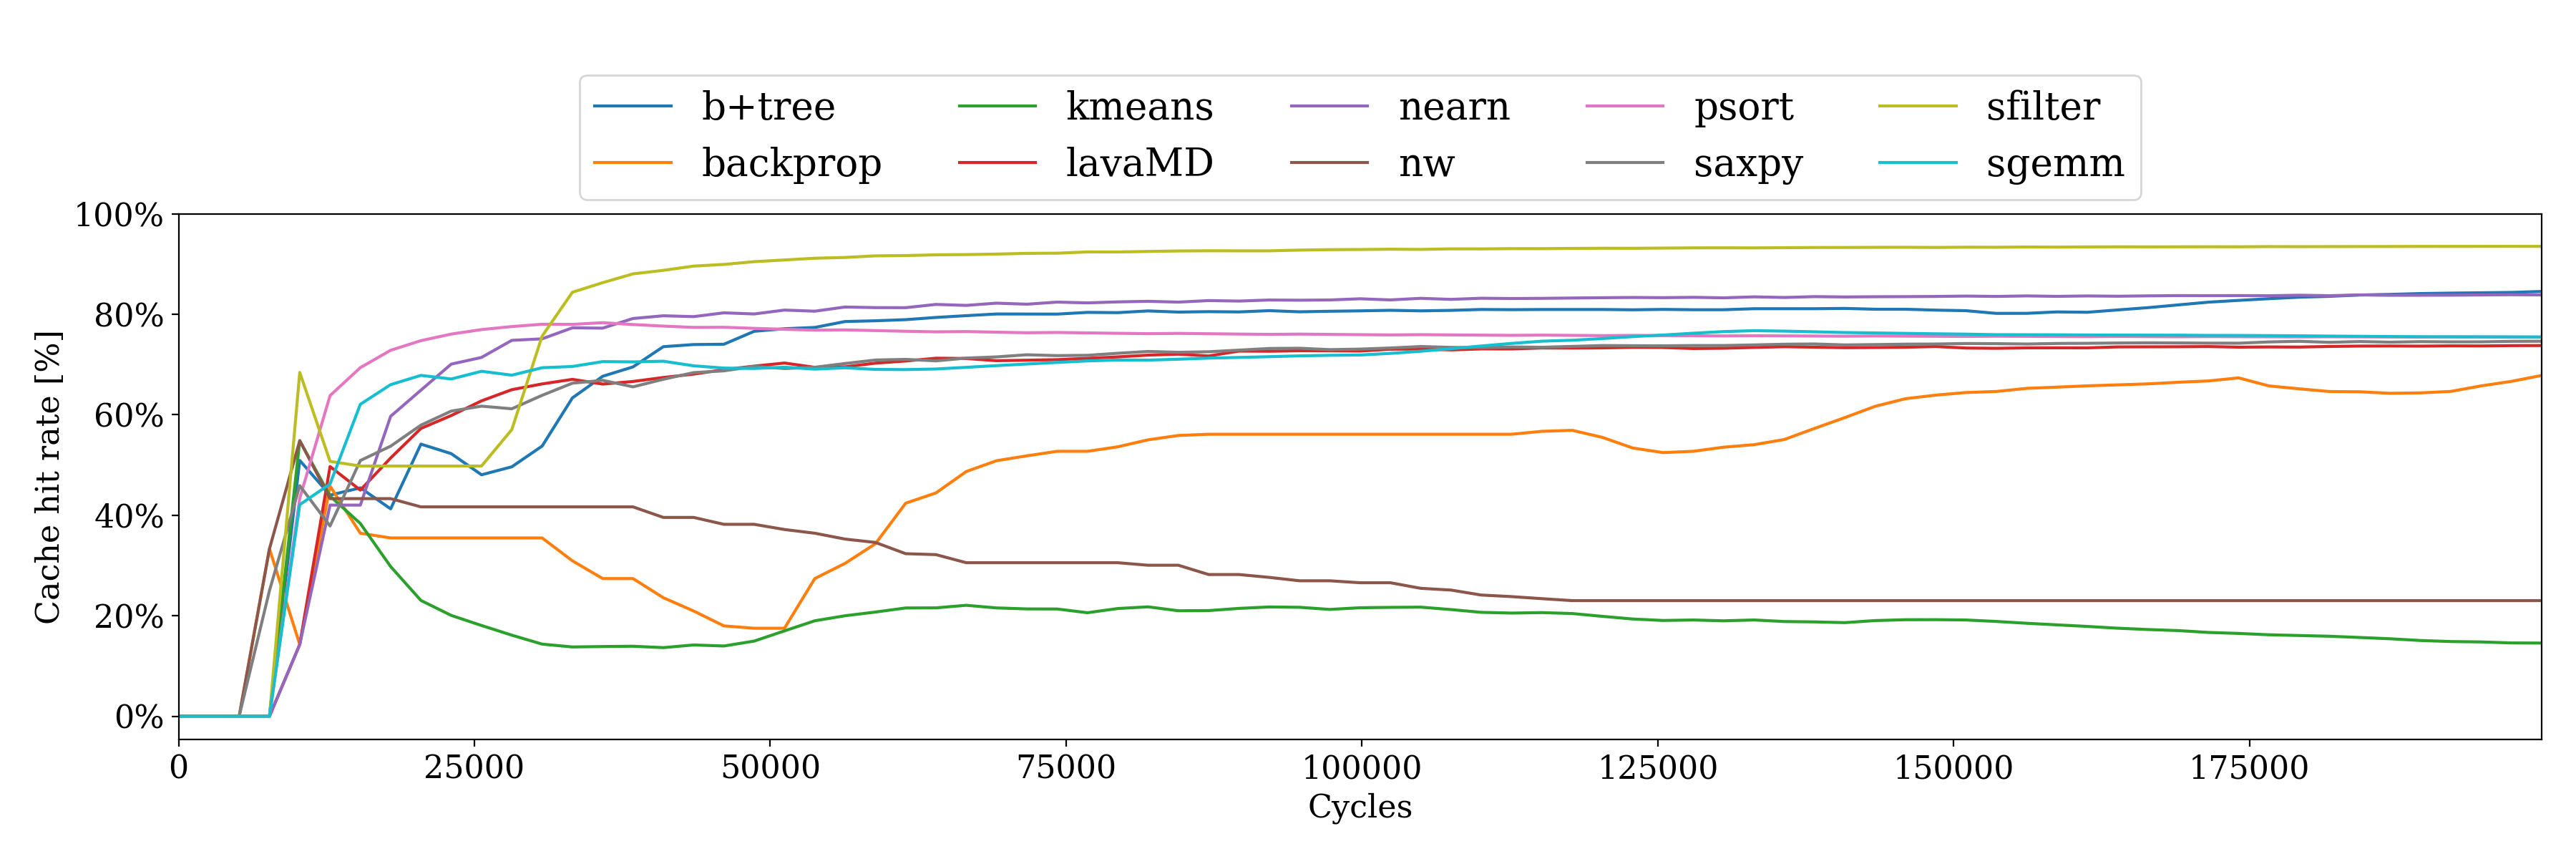
\includegraphics[width=\textwidth]{figures/L1cachehit_vlsim.png}
        \caption{L1 dcache hit rate during startup}
        \label{fig:l1_cache_startup_hitrate}
    \end{subfigure}
    \hfill
    \begin{subfigure}[t]{\textwidth}
        \centering
        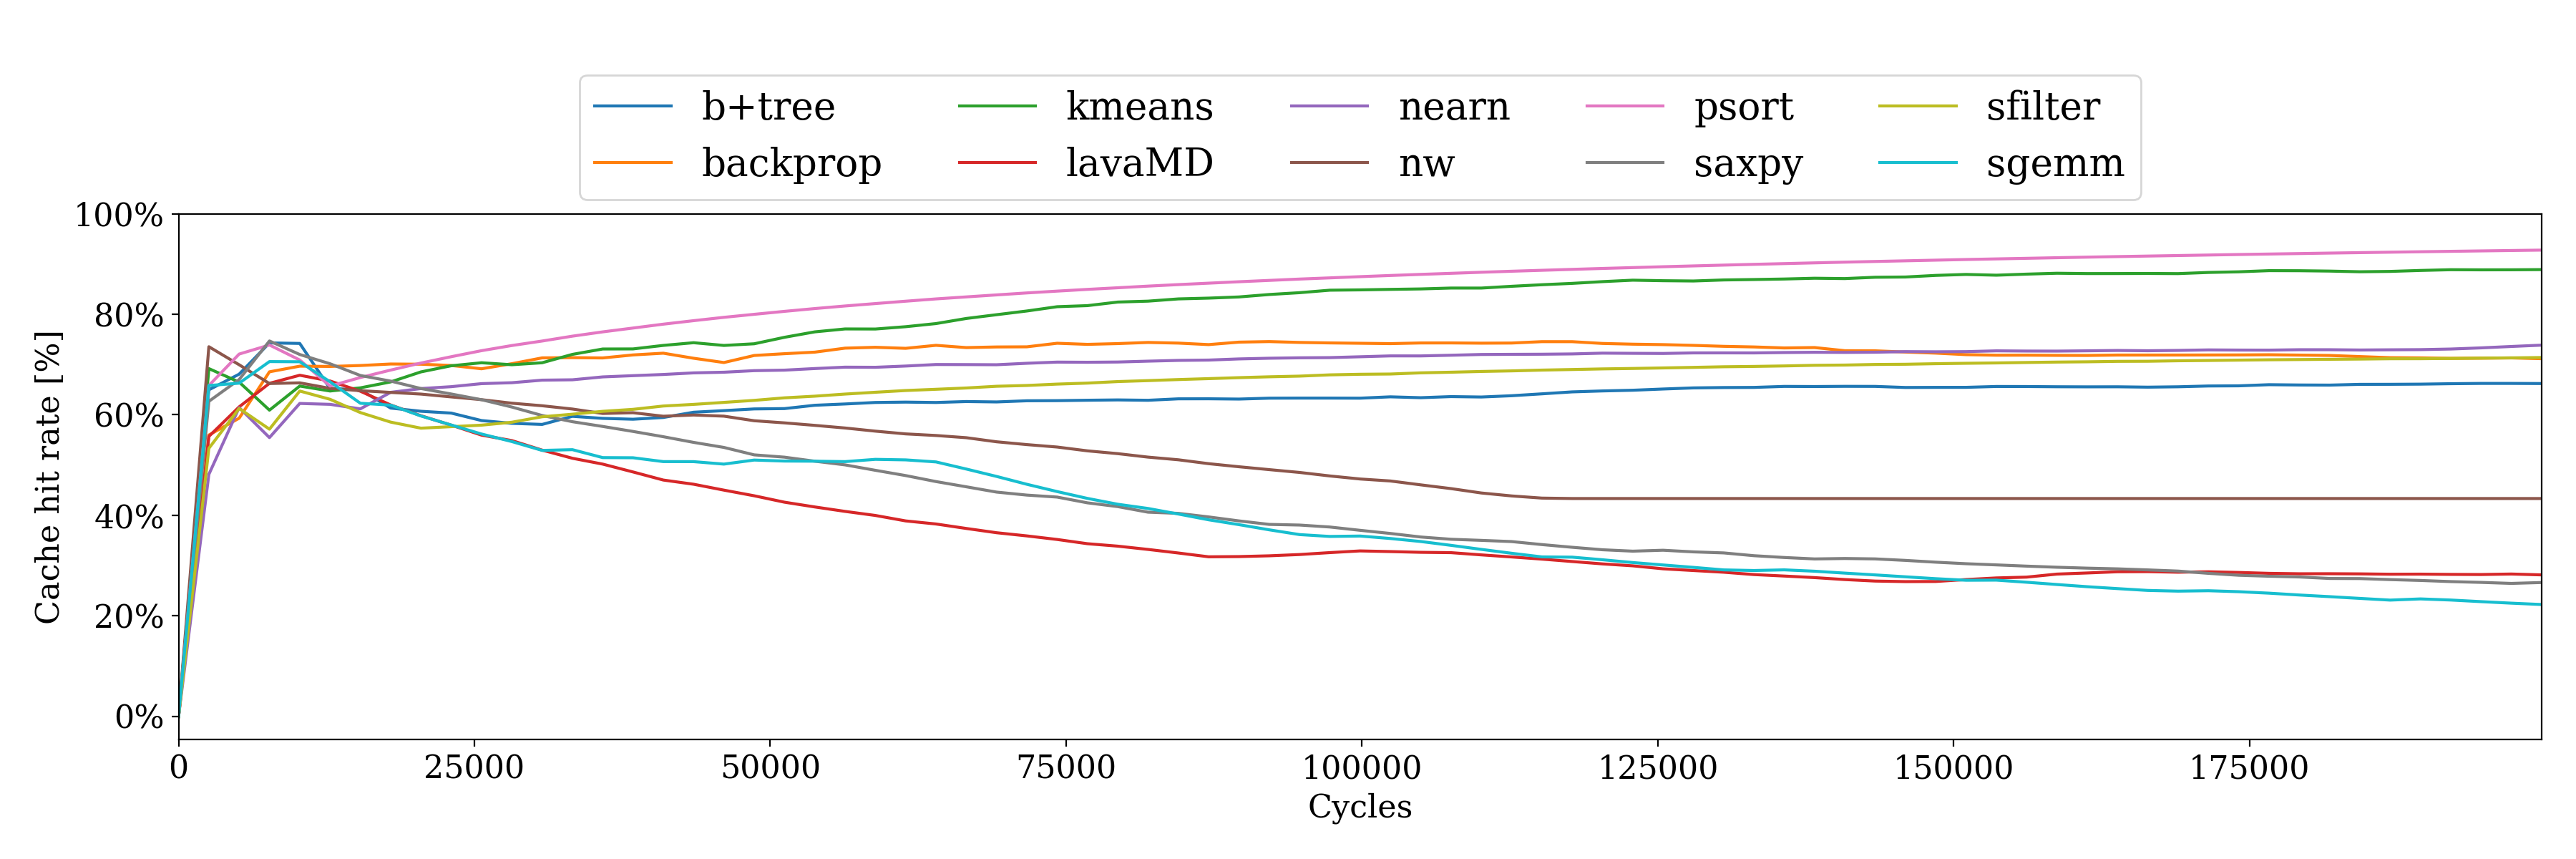
\includegraphics[width=\textwidth]{figures/L2cachehit_vlsim.png}
        \caption{L2 dcache hit rate during startup}
        \label{fig:l2_cache_startup_hitrate}
    \end{subfigure}
    \caption[Dcache hit rates over time during startup.]{Dcache hit rates over time for a subset of the benchmarks during startup.}
    \label{fig:dcache_startup_hitrate}
\end{figure}

\section{IDUN Cluster}

All the simulations were run on the IDUN Cluster~\cite{Idun_tech_report} at NTNU. Running the simulations required a substantial amount of time and memory. The total compute time required to run all the simulations scales with the number of benchmarks. Adding 16 new benchmarks thus increase the total simulation time significantly. Using IDUN allowed me to run all benchmarks in parallel, thus saving a lot of time, as most benchmarks required many hours to complete.
\newpage
The installation of \Gls{vortex} had to be modified due to missing permissions to write to some of the install locations. It also followed that the locations of these dependencies had to be changed in the \Gls{vortex}' makefiles.

Unfortunately, there were some discrepancies when running some of the benchmarks on IDUN. The results of \textit{LUD}, \textit{SRAD} were drastically different when simulated on my personal machine and on IDUN. I was also unable to run \textit{particle filter} on IDUN without crashing, although it executed without errors on my personal machine. I was unable to identify any specific reasons for these discrepancies, but it could be due to differences in software or library versions. Because of this, these benchmarks are not included in the results in Chapter~\ref{chap:results}.